%\documentclass[iop]{emulateapj}
\documentclass[aps, prl, twocolumn, groupedaddress]{revtex4-1}
\usepackage{amsmath}
\usepackage{graphicx}
\usepackage{epstopdf}
\usepackage{listings}
\usepackage{color}
\usepackage{bm}
\usepackage{empheq}
\usepackage{natbib}
\usepackage{cancel}
\usepackage[colorlinks=True, linkcolor=blue, citecolor=blue]{hyperref}
\usepackage[all]{hypcap}

\bibliographystyle{apsrev}

\newcommand{\Div}[1]{\ensuremath{\nabla\cdot\left( #1\right)}}
\newcommand{\angles}[1]{\ensuremath{\left\langle #1 \right\rangle}}
\newcommand{\grad}{\ensuremath{\nabla}}
\newcommand{\RB}{Rayleigh-B\'{e}nard }
\newcommand{\stressT}{\ensuremath{\bm{\bar{\bar{\Pi}}}}}


\begin{document}
%%%%% Create nice title and abstract
\author{Evan H. Anders}
\affiliation{Department of Astrophysical \& Planetary Sciences, University of Colorado -- Boulder}
\affiliation{Laboratory for Atmospheric and Space Physics, Boulder, CO}
\author{Benjamin P. Brown}
\affiliation{Department of Astrophysical \& Planetary Sciences, University of Colorado -- Boulder}
\affiliation{Laboratory for Atmospheric and Space Physics, Boulder, CO}
\title{Convective heat transport in stratified atmospheres at low and high Mach number}

\begin{abstract}
This is where an abstract defining what we're doing with stratified convection and Nusselt numbers will go.
\end{abstract}
\maketitle


%%%%% Body of the paper
\section{Introduction \label{section:intro}}
Convection is ubiquitous among natural systems such as stellar envelopes and planetary atmospheres.
Compressible convection in such stratified atmospheres exhibits behavior which is much more complex than 
what is seen in the widely-studied \RB convection.  Upflows and downflows are asymmetric, the well-defined
Rayleigh Number (Ra, the ratio of buoyant driving to diffusive damping) becomes less defined and depth-dependent,
and the Mach number of the flows becomes an additional control parameter.
Early studies of stratified
convection in two \cite{graham1975, chan&all1982, hurlburt&all1984, cattaneo&all1990} and three 
\cite{malagoli&all1990, cattaneo&all1991, brummell&all1996} dimensions
utilized polytropically stratified atmospheres, in which the temperature gradient, thermal diffusivity, and
gravity are constant throughout the depth of the atmosphere and the atmosphere is initially in hydrostatic equilibrium.
While often abandoned for atmospheres constructed using more realistic
radiative transfer properties (cite some papers), the polytrope is a particularly useful reference state for
stratified convection studies.

A canonical value of the ``polytropic index'' used in the study of convection of monatomic ideal gases is
$m = 1$, such that the density and temperature profile are both linear.  Recently, \cite{brandenburg&all2005}
argued that as the polytropic index approaches the adiabatic value of $m_{ad} = 1.5$, the convective flux of
the system becomes negligible compared to the background flux gradient, and the Nusselt number of the
system approaches zero.  They argue that, as a result, values of $m \rightarrow -1$ are ideal polytropes
to study, as the radiative flux approaches zero and the convective flux carries the whole of the system
flux in equilibrium. 

Here, we argue for The definition of a new Nusselt number, where the radiative flux is defined relative to
the \emph{adiabatic} state rather than to a linear temperature profile.  We demonstrate that values
of $m$ close to adiabatic show a Nusselt number (similar?) to \cite{johnston&doering2009} and that
such values of $m$ are useful in allowing us to probe low-Mach number convection, such as that
deep within the Sun's convection zone (cite a paper for that?)


\section{Model \& Equations \label{section:model}}
We study a fluid whose equation of state is that of an ideal gas, $P = R^*\rho T$ and whose
initial stratification is polytropic, where
\begin{equation}
\begin{split}
\rho_0(z) &= \rho_{00}(z_0 - z)^m \\
T_0(z)    &= T_{00}(z_0 - z)
\label{eqn:polytrope}
\end{split}
\end{equation}
and $z$ increases upwards within the bounds $z =\{0, L_{z}\}$.
The height of the atmosphere is set by specifying the number of density scale heights it spans, $n_\rho$,
which we set to be three throughout this study such that the density at the bottom of the atmosphere is larger
than that at the top of the atmosphere by roughly a factor of 20.
Variables are nondimensionalized at the top of the atmosphere as 
$P_0(L_z) = \rho_0(L_z) = T_0(L_z) = 1$, requiring $z_0 \equiv L_z + 1$ and $R^* = T_{00} = \rho_{00} = 1$.  
The polytropic index is set by the adiabatic index of a monatomic ideal gas, $\gamma = 5/3$ and the 
control parameter $\epsilon$, such that $m = (\gamma - 1)^{-1} - \epsilon = m_{ad} - \epsilon$ 
and the subsequent entropy gradient at the top of the atmosphere is $\grad S(L_z) = -\epsilon$.

The primary assumptions utilized in constructing a polytropic atmosphere are that acceleration due to 
gravity is constant and that the conductive heat flux, $F_{\text{cond}} = -\kappa \grad T_0$ is
constant throughout the atmosphere.  To ensure the second condition is met, it is traditional to use
a constant value of $\kappa$ and $\grad T_0$.  The thermal conductivity is controlled by the
non-dimensional Rayleigh number,
\begin{equation}
\text{Ra} = \frac{g L_z^3 (\Delta S_0 / c_P)}{\nu\chi},
\end{equation}
where $\Delta S_0$ is the entropy jump across the polytropic atmosphere, $\nu$ is the kinematic viscosity
and $\kappa$ is the thermal diffusivity.  The relationship between the thermal and viscous diffusivities is
set by the Prandtl number, Pr$ = \nu/\chi$, which we take to be one throughout this study.   The thermal
and viscous diffusion coefficients are related to the dynamic viscosity, $\mu$ and $\kappa$ by the ratio
$\nu \equiv \mu/\rho$ and $\chi \equiv \mu\/rho$.  As a result, $\text{Ra} \propto (\nu\chi)^{-1} \propto
\rho^2$, such that for our atmospheres with $n_{\rho} = 3$, the Rayleigh number increases by a factor of
approximately 400 from the top of the domain to the bottom of the domain.

At the constant values of $n_\rho$ and Pr used, the primary control parameters of convection are $\epsilon$
and Ra.  We decompose our atmosphere into the background polytrope ($\rho_{0}, T_{0}$) and the fluctuations
about that background ($\bm{u}, \rho_{1}, T_{1}$).  The scaling of the entropy gradient with $\epsilon$
is reflected in the evolved values of these fluctuations, which follow the scaling of
Ma$^{1/2} \propto T_1/T_0 \propto \rho_{1}/\rho_{0} \propto \epsilon$, and which scale weakly with Ra (prove it,
we have the data). 

\begin{figure}[t]
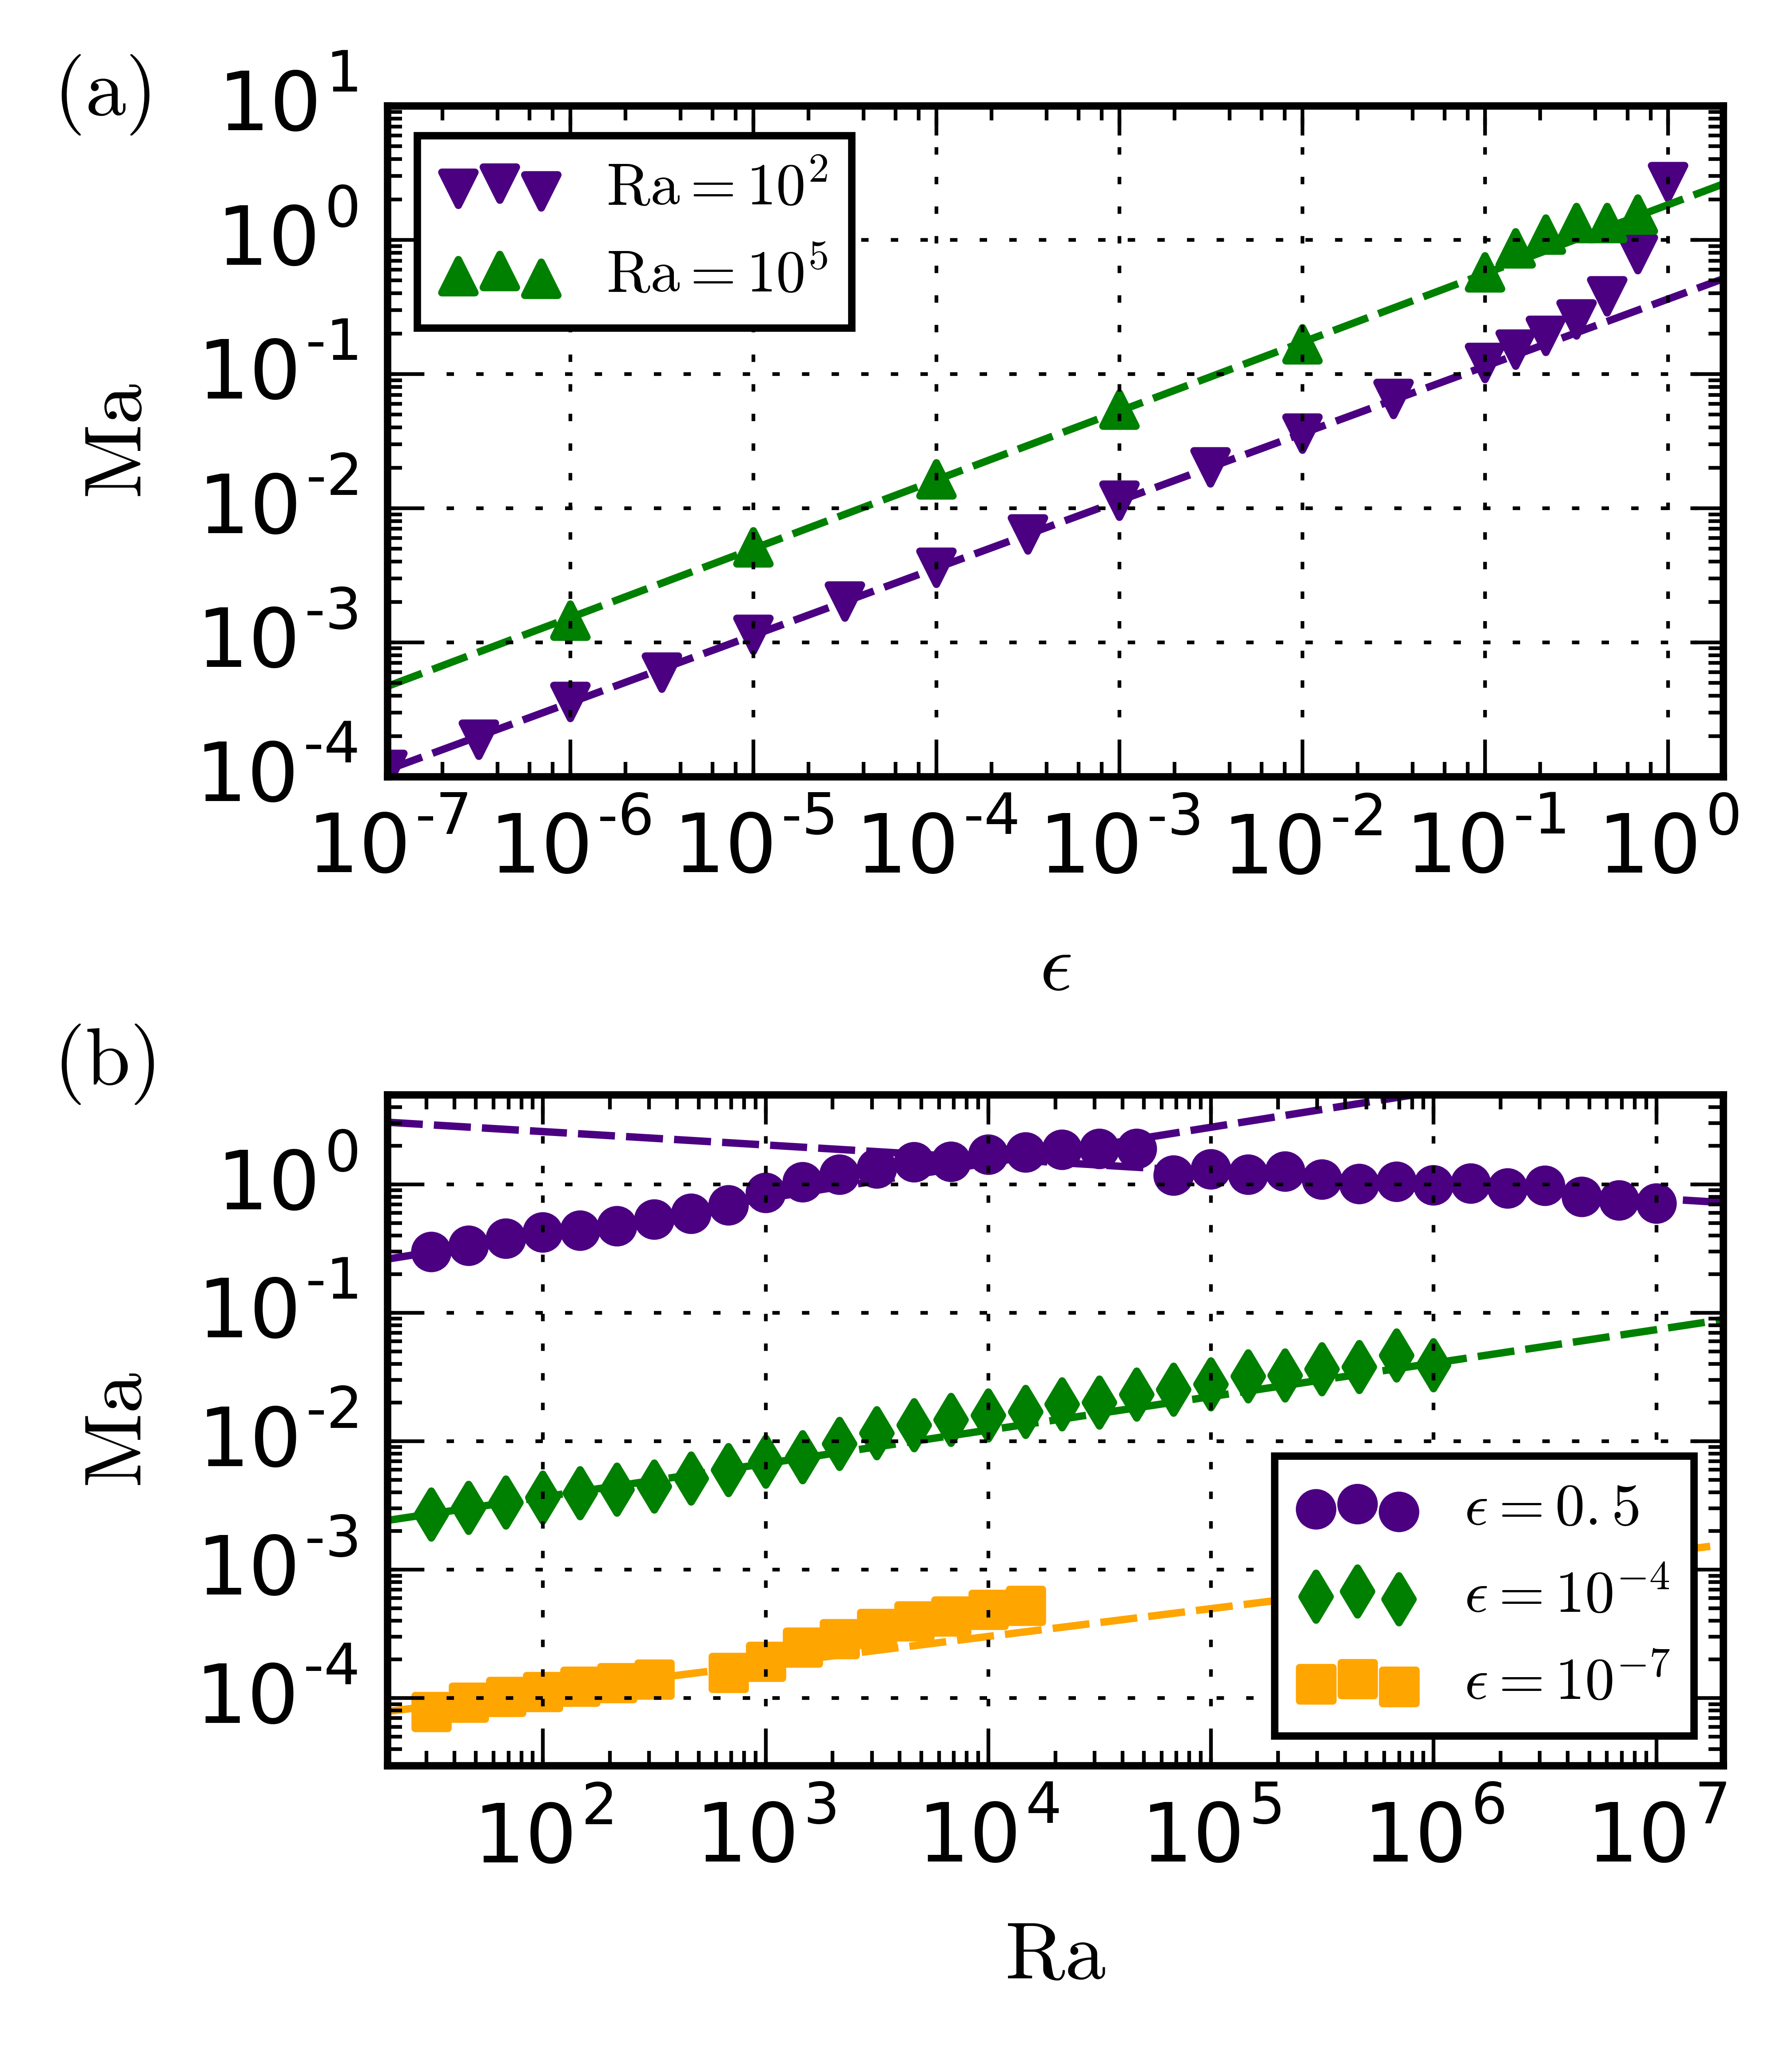
\includegraphics[width=3.5in]{./figs/ma_v_eps.eps}
\caption{Shown are characteristic mach numbers from IVPs spanning six decades of $\epsilon$, from
very low Mach number to near Mach one.  A very strong Ma $\propto \epsilon^{1/2}$ relation is clear. 
(need to actually do linear regression)
\label{fig:ma_v_eps} }
\end{figure}



We start with initial conditions of random small perturbations compared to $\epsilon$ in the temperature
field.  We evolve the Fully Compressible Navier-Stokes equations with an energy-conserving energy equation,
which take the form:
\begin{align}
&\begin{aligned}
&\frac{D \ln\rho}{D t} + \Div{\bm{u}} = 0
	\label{eqn:continuity_eqn}
\end{aligned}\\
&\begin{aligned}
&\rho\frac{D\bm{u}}{D t}=
-\grad P + \rho\bm{g} - \nabla\cdot\stressT
	\label{eqn:momentum_eqn}
\end{aligned}\\
&\begin{aligned}
\rho c_V\left(\frac{D T}{D t} + (\gamma-1)T\Div{\bm{u}}\right) + &\Div{-\kappa\grad T} = \\
&-\left(\stressT\cdot\nabla\right)\cdot\bm{u} 
	\label{eqn:energy_eqn}
\end{aligned}
\end{align}
where $D/Dt \equiv \partial_t + \bm{u}\cdot\grad$ and the viscous stress tensor is defined as
\begin{equation}
\Pi_{ij} \equiv -\mu\left(\frac{\partial u_i}{\partial x_j} + \frac{\partial u_j}{\partial x_i} - \frac{2}{3}\delta_{ij}\Div{\bm{u}}\right).
	\label{eqn:stress_tensor}
\end{equation}

In such stratified systems, the total convective flux can be defined as
\begin{equation}
\bm{F}_{\text{conv}} = \bm{F}_{\text{enth}} + \bm{F}_{\text{KE}} + \bm{F}_{\text{PE}} + \bm{F}_{\text{visc}},
\end{equation}
where $\bm{F}_{\text{enth}} \equiv \rho\bm{u}(c_V T + P/\rho)$ is the enthalpy flux, $\bm{F}_{\text{KE}} \equiv 
\rho|\bm{u}|^2\bm{u}$ is the kinetic energy flux, $\bm{F}_{\text{PE}} \equiv \rho\bm{u}\phi$ is the potential
energy flux (with $\phi \equiv -gz$), 
and $\bm{F}_{\text{visc}} \equiv \bm{u}\cdot\stressT$ is the viscous flux.  Dotting 
Eq. \ref{eqn:momentum_eqn} with $\bm{u}$ and adding it to 
Eq. \ref{eqn:energy_eqn}, we retrieve the full energy equation in conservation form,
\begin{equation}
\frac{\partial}{\partial t}\left(\rho\left[\frac{|\bm{u}|^2}{2} + c_V T + \phi\right]\right) +
\Div{\bm{F}_{\text{conv}} + \bm{F}_{\text{rad}}} = 0
	\label{eqn:energy_eqn_full}
\end{equation}
where $\bm{F}_{\text{rad}} = -\kappa \grad T$. 

The efficiency of convection is defined by the Nusselt number.  While the Nusselt number is well-defined in \RB convection
as the amount of total flux divided by the steady-state background conductive flux 
\cite{johnston&doering2009, otero&all2002},
a well-defined Nusselt number is more elusive in stratified convection.  Convection generally 
works to drive the overall \emph{entropy} gradient to zero.  In the case of the Boussinesq approximation of
\RB convection, $\grad S = 0$ implies that $\grad T = 0$ because density is no longer a factor in determining the
stratification.  However, once compressibility and stratification are considered, convection works to cause
$\grad S = 0$ but \emph{not} necessarily $\grad T = 0$.  As such, even perfectly efficient convection will still
have some amount of adiabatic conductive flux, $F_A \equiv -\kappa \grad T_{ad}$.  In the case of an initially
superadiabatic polytrope, assuming that hydrostatic equilibrium is conserved to first order and that the system
evolves towards a new, adiabatic polytropic state such that the temperature gradient takes the form
$\grad T_{\text{ad}} = -g/c_P = \grad T_0 (1 - \epsilon(m_{ad} + 1))$.  In order to obtain a meaningful definition
of the conductive flux, this constant adiabatic component must be subtracted, which yields
$\bm{F}_{\text{rad}} - \bm{F}_{\text{ad}} = -\kappa\grad T_1 -\kappa\grad T_0\epsilon(m_{ad} + 1)$.  Unlike
the full radiative flux, which is $O(\kappa\grad T)$, this is $O(\kappa\grad T_1) \approx O(\epsilon)$, and it
is thus comparable to the other fluxes in the system, as would be expected.  Acknowledging this, we define the
Nusselt number in the same form as \cite{hurlburt&all1984}, who wrote it as
\begin{equation}
N \equiv \frac{F_{\text{conv, z}} + F_{\text{rad, z}} - F_A}{F - F_A},
\label{eqn:nusselt}
\end{equation}
where $F = \Delta T / Lz$ is the radiative flux carried by a
linear temperature profile from the top boundary value to the bottom boundary value.
It is important to note that such a definition explains the results of \cite{brandenburg&all2005}, who noted that
as $m \rightarrow -1$, $F_{\text{rad}}\rightarrow 0$ and $F_{\text{conv}}$ becomes large.  As $m\rightarrow -1$,
$g\rightarrow 0$, such that the adiabatic flux become zero and the Nusselt number definition reverts to a form
more similar to that of \RB convection.

***WE USE DEDALUS, EXPLAIN WHAT IT ARE***

***EXPLAIN BOUNDARY CONDITIONS***

***EXPLAIN WHAT THE CHARACTERISTIC TIME SCALE, THE BUOYANCY TIME, IS***


\section{Results \label{section:results}}
We ran initial value problems for a few hundreds of buoyancy times past the convective transients from 
Rayleigh numbers around $R_{crit}$ up to Rayleigh numbers of $\approx 10^7 R_{crit}$.  While bulk thermodynamic
structures are similar between low and high $\epsilon$, high $\epsilon$ runs start to exhibit shock fronts
propagating away from downflow channels, such as those in Fig. \ref{fig:entropy_snapshots}, as reported in
(cite Juri's paper from ~1990 that has this).
\begin{figure}[t]
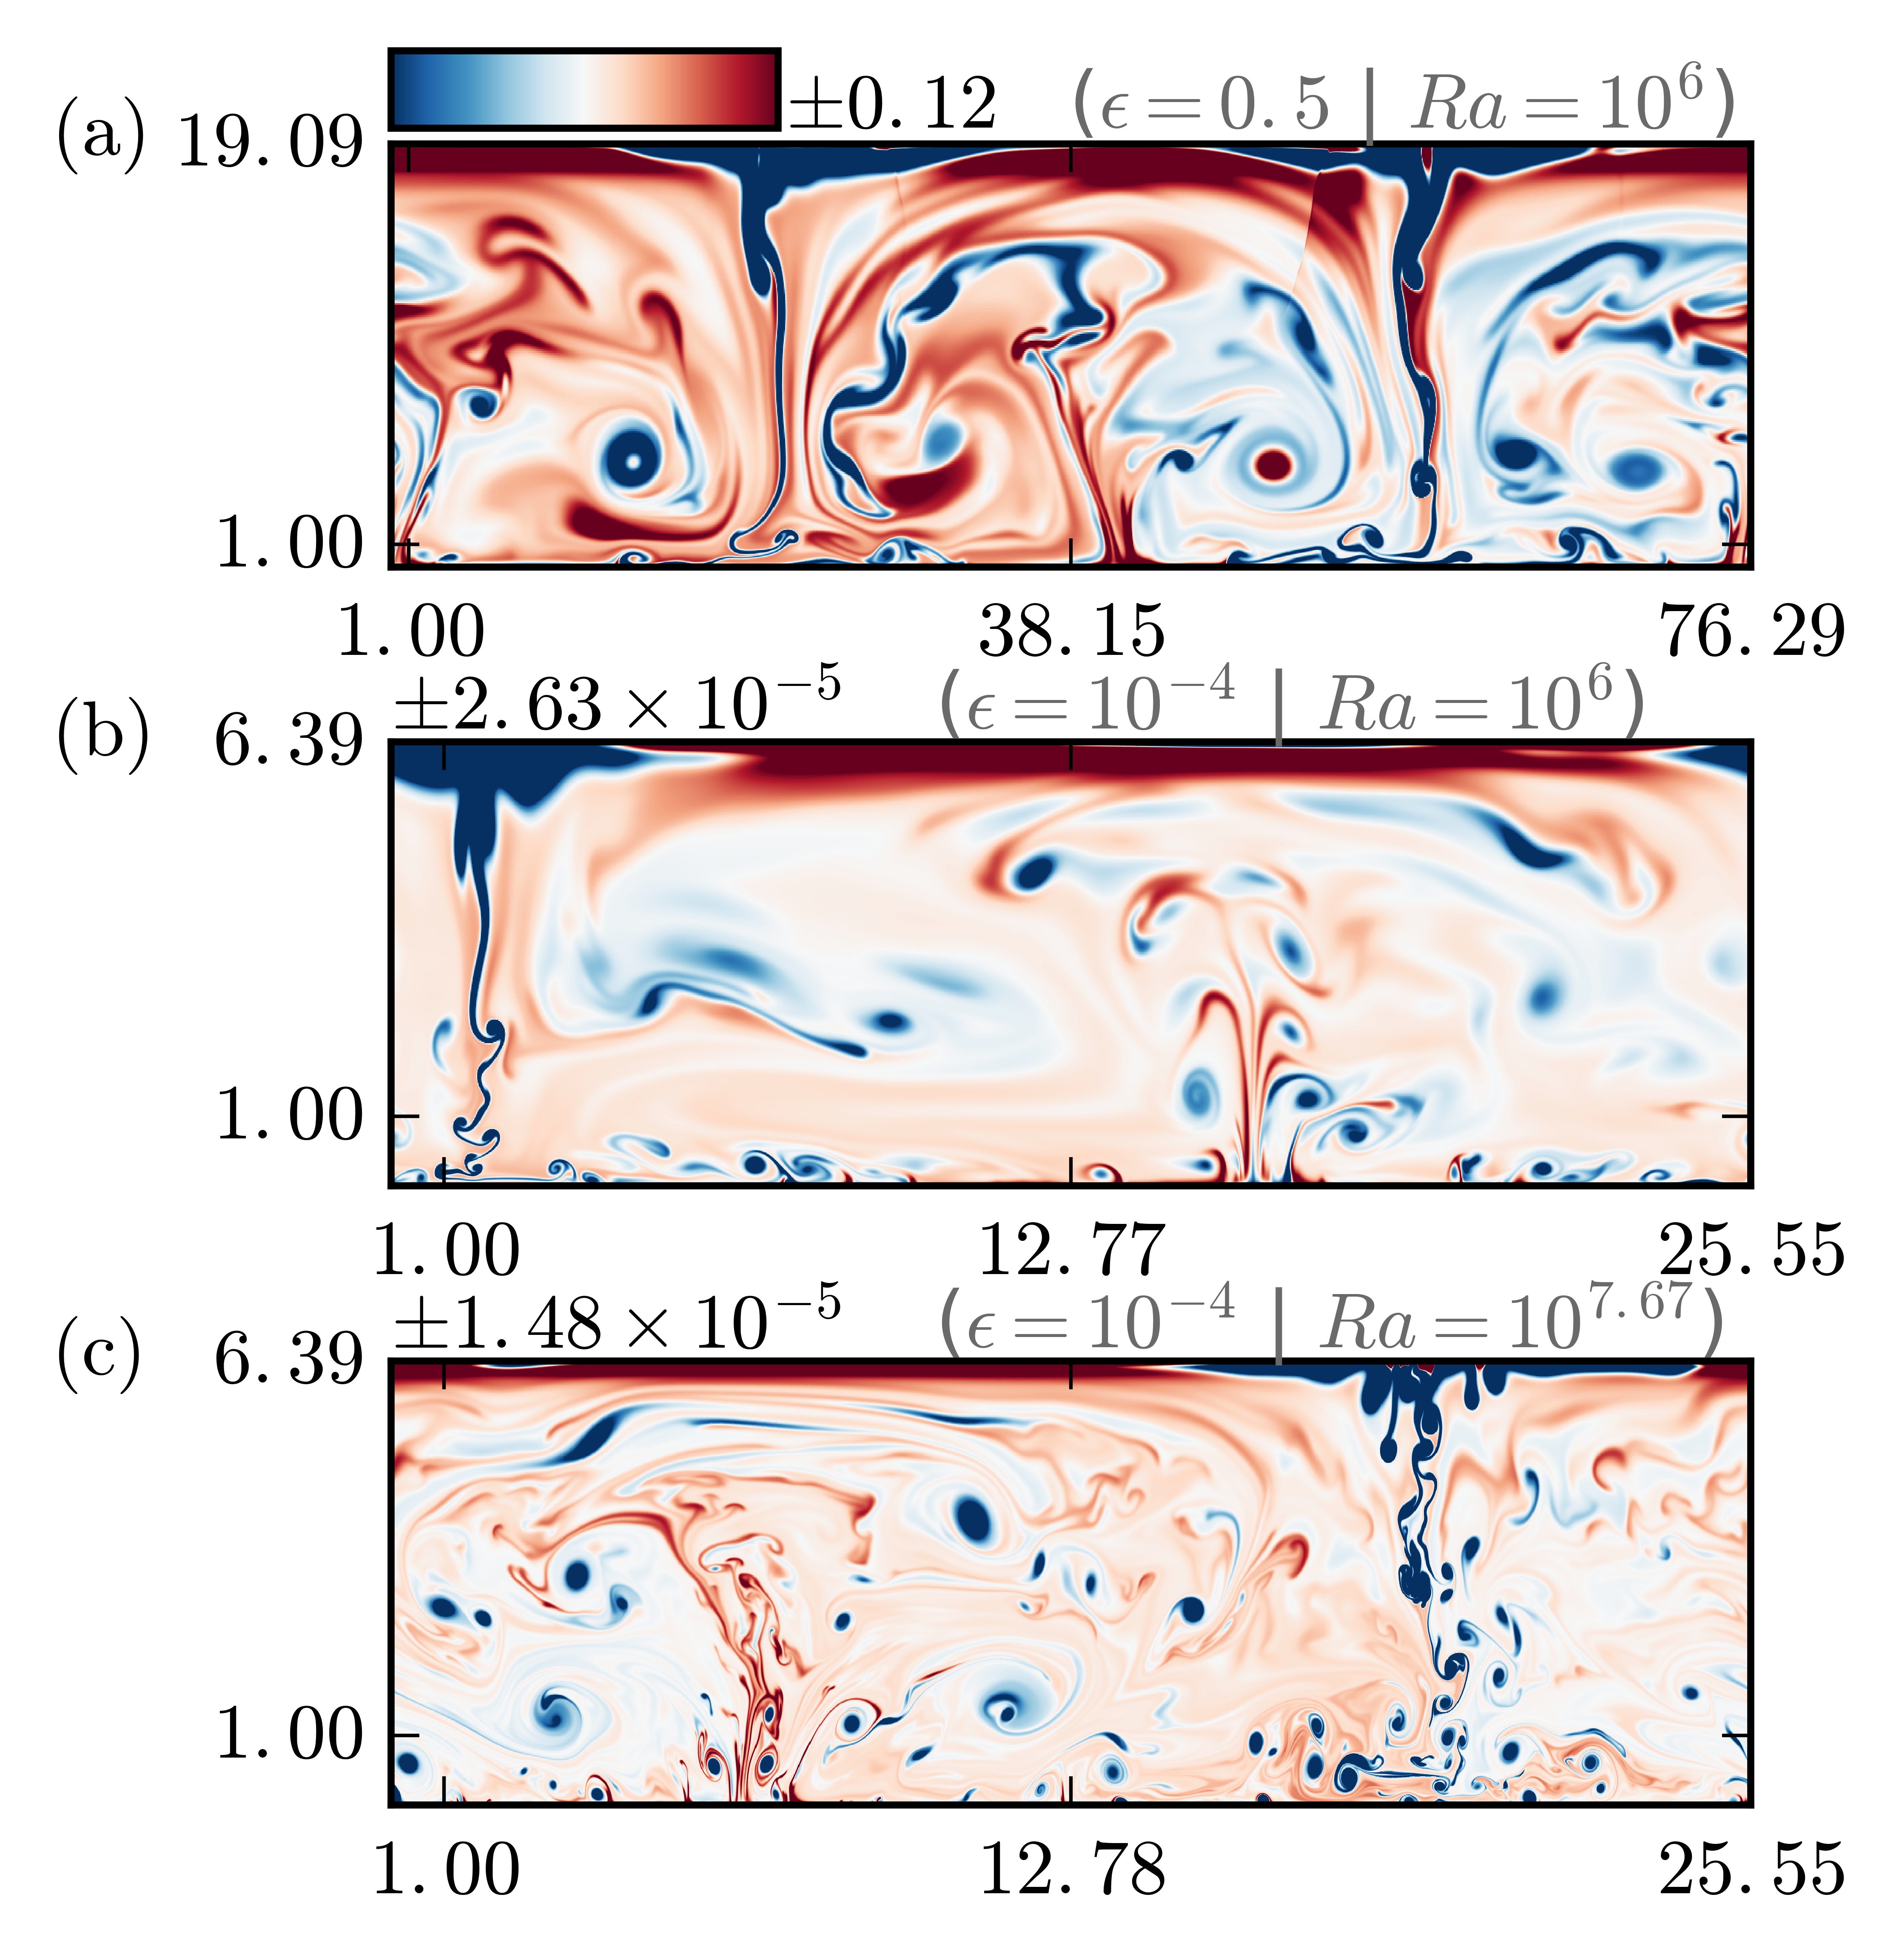
\includegraphics[width=3.5in]{./figs/snapshots_fig.eps}
\caption{Two characteristic snapshots after about 200 buoyancy times are shown at $\epsilon=10^{-4}$ (top)
and $\epsilon=0.5$ (bottom) at Ra = $10^6$.  
\label{fig:entropy_snapshots} }
\end{figure}

Despite diferent thermodynamic structures, the fluxes look fairly similar at low and high mach number (sort of?
I don't think the ones I have are averaged over enough time, especially the eps=0.5 one, but I Pleiades is
a bit slammed right now).  See Fig \ref{fig:flux_profiles}

\begin{figure}[b]
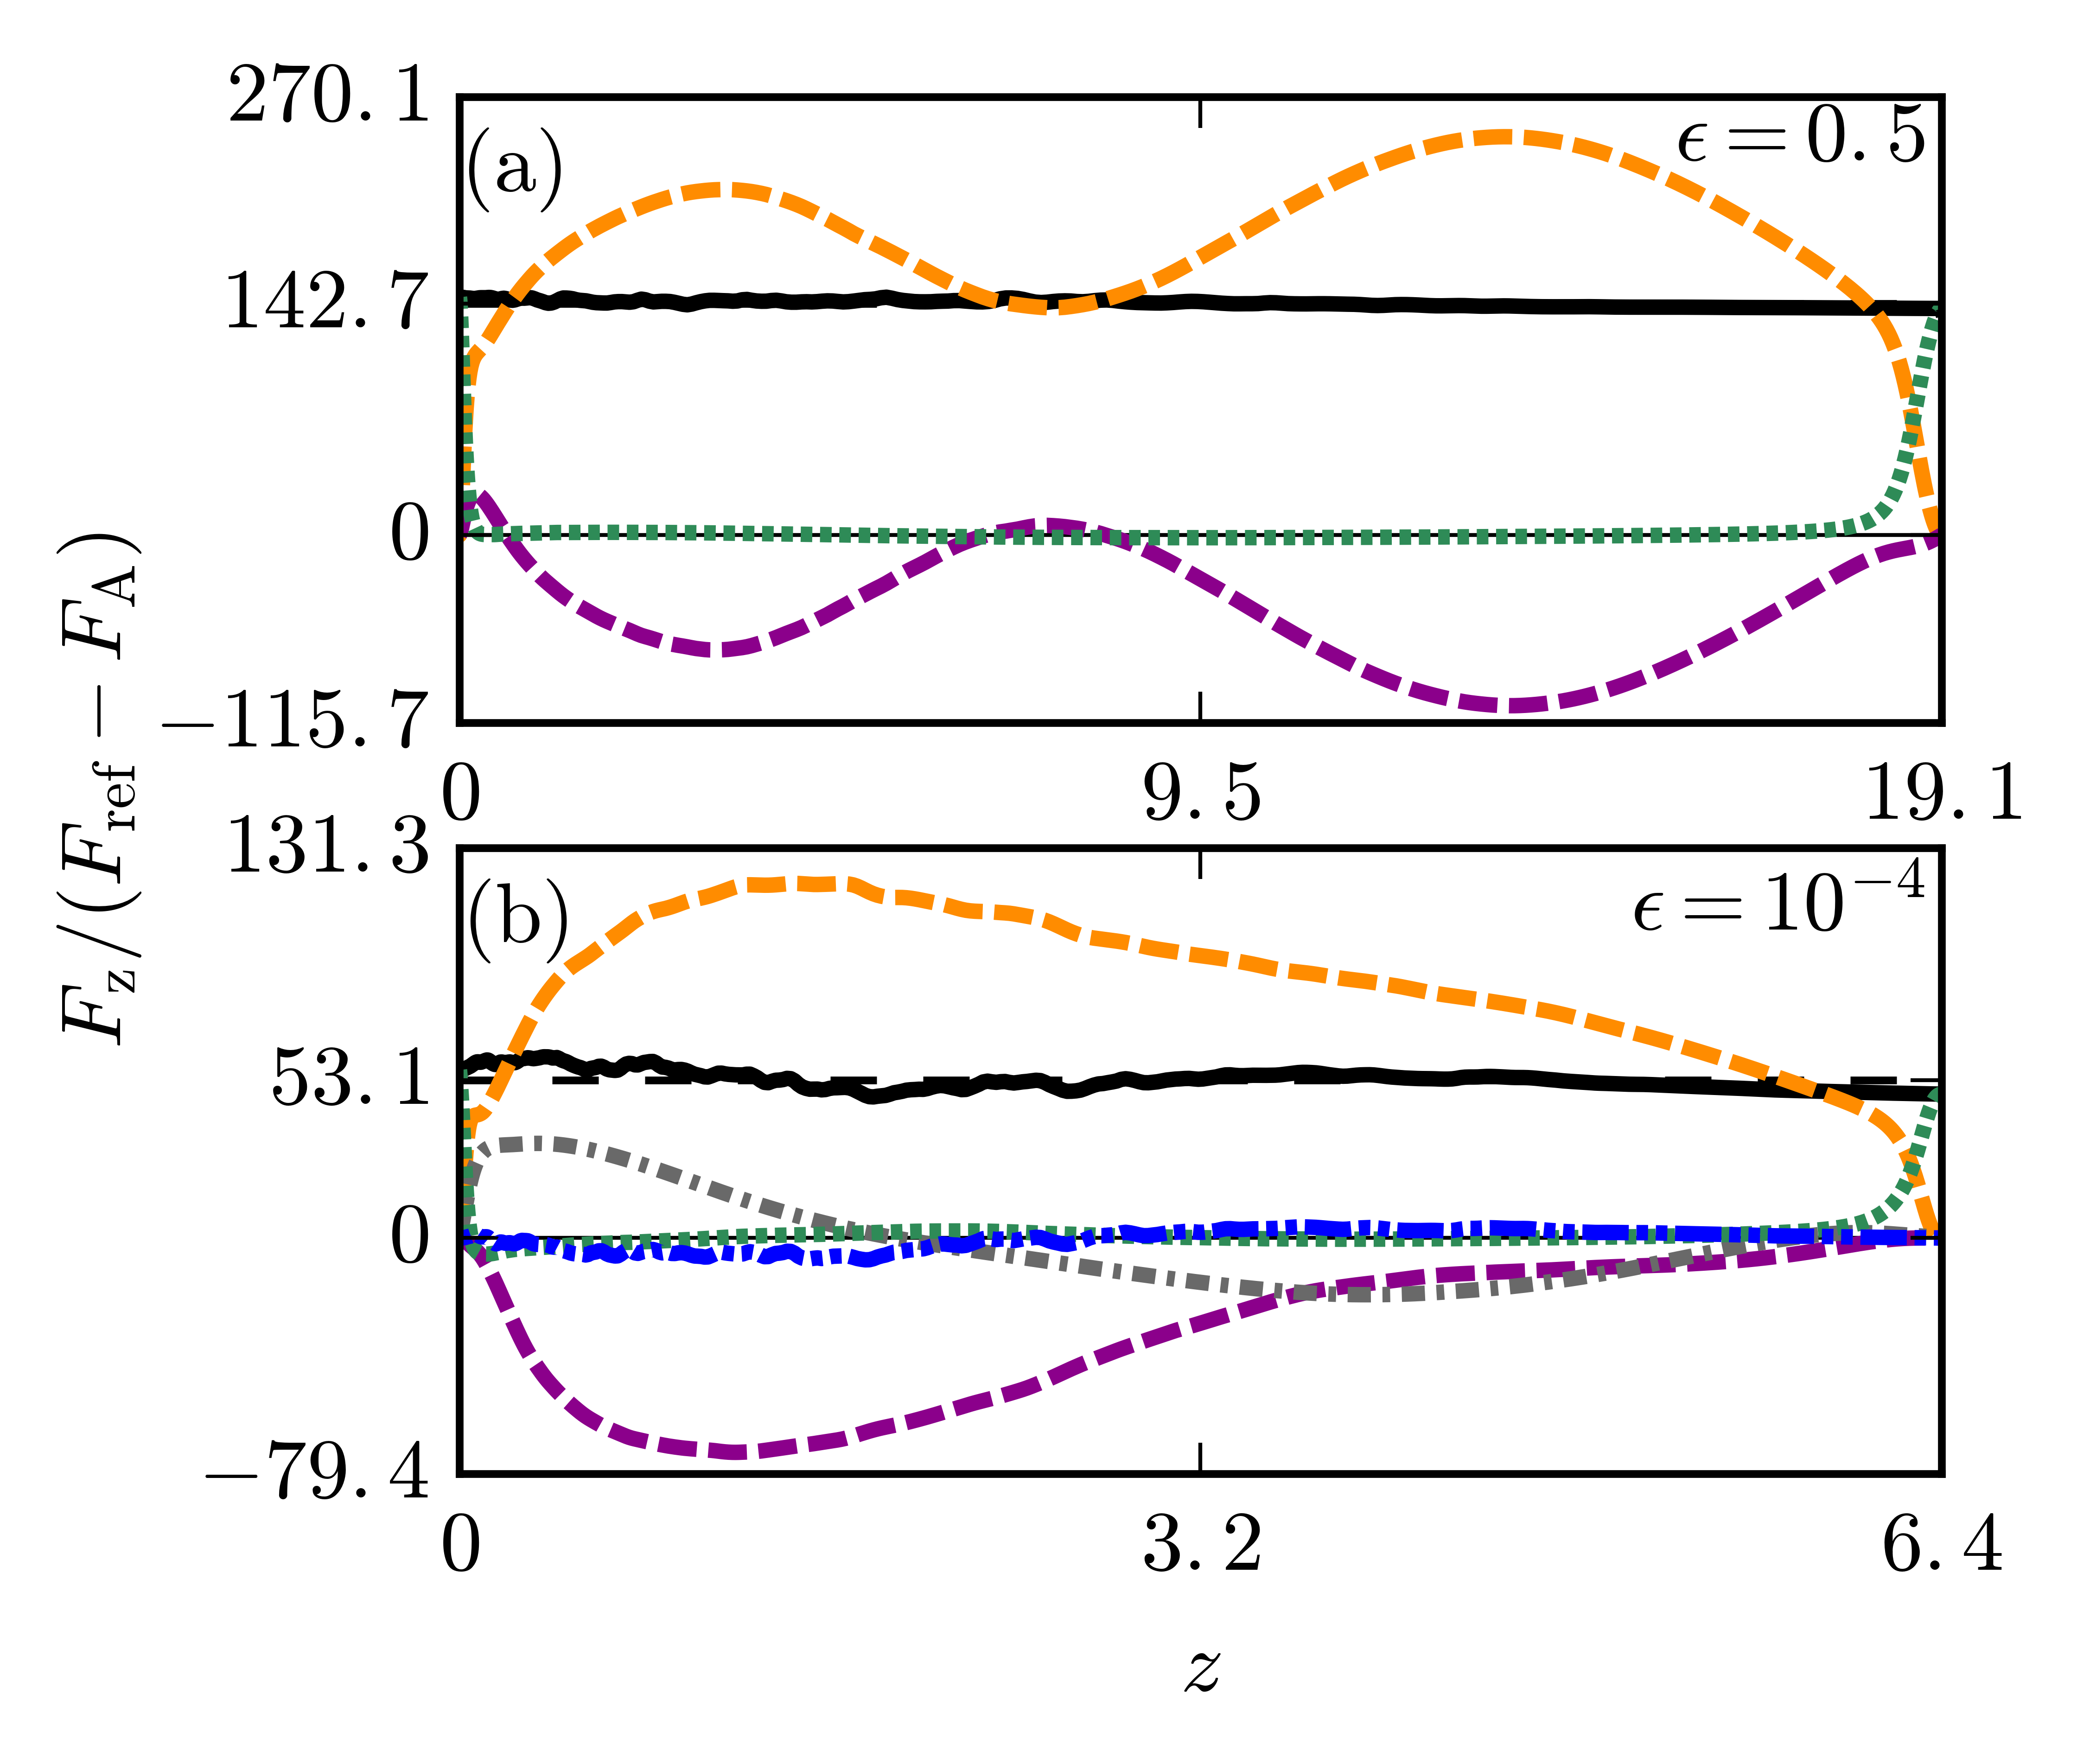
\includegraphics[width=3.5in]{./figs/fluxes_fig.eps}
\caption{Flux profiles for low (top) and high (bottom) Mach number flows.  
\label{fig:flux_profiles} }
\end{figure}

At low Rayleigh number, diffusivities are high and the flows are very laminar.  Such flows often achieve a
steady state and have a well-defined Nusselt number which is independent of time.  However, as the Rayleigh
number increases, the flows become increasingly time-dependent.  Even steady structures such as solid
``rolls'' like those pictured in Fig. \ref{fig:entropy_snapshots} have highly time-dependent Nusselt numbers.
This is, in part, due to the fact that cold downdrafts floating to the bottom of the domain can be entrained
by upflows, or warm risen parcels can be entrainedi n the intense cold downdrafts.  Such events reverse the
preferred direction of flux in the system, and even let the Nusselt number become negative for short periods of
time.  See Fig. \ref{fig:nu_v_time}.  As a result, it is necessary to take a long time average of the fluxes
before calculating the Nusselt number at higher Rayleigh number.


\begin{figure}[t]
\includegraphics[width=3.5in]{./figs/nu_v_time.eps}
\caption{The evolution of the Nusselt number is shown at low ($10^2$) and high ($10^7$) Rayleigh number and at
$\epsilon = 10^{-4}$.  At low Rayleigh number, the system is able to settle into a time invariant solution. As
the Rayleigh number is raised, the thermodynamic structure become increasingly complex and time variant, and a
time-average of the Nusselt number is required to obtain a sensible mean.
\label{fig:nu_v_time} }
\end{figure}

The evolution of the Nusselt number as the Rayleigh number is increased is shown for both high and low
$\epsilon$ in Fig. \ref{fig:nu_v_ra}.  Below convective onset, the Nusselt number is perfectly one. Just above
onset, there is a brief range of highly inflated scaling between $N$ and Ra.  From about $10R_{crit}$ to roughly
$10^{4-5}R_{crit}$, Ra and $N$ follow the relationship: (put a power law here)  Above about
$10^5 R_{crit}$, the Nusselt number flattens out as Ra is increased -- perhaps this is some Featherstone 2016
shennanigans.

\begin{figure}[b]
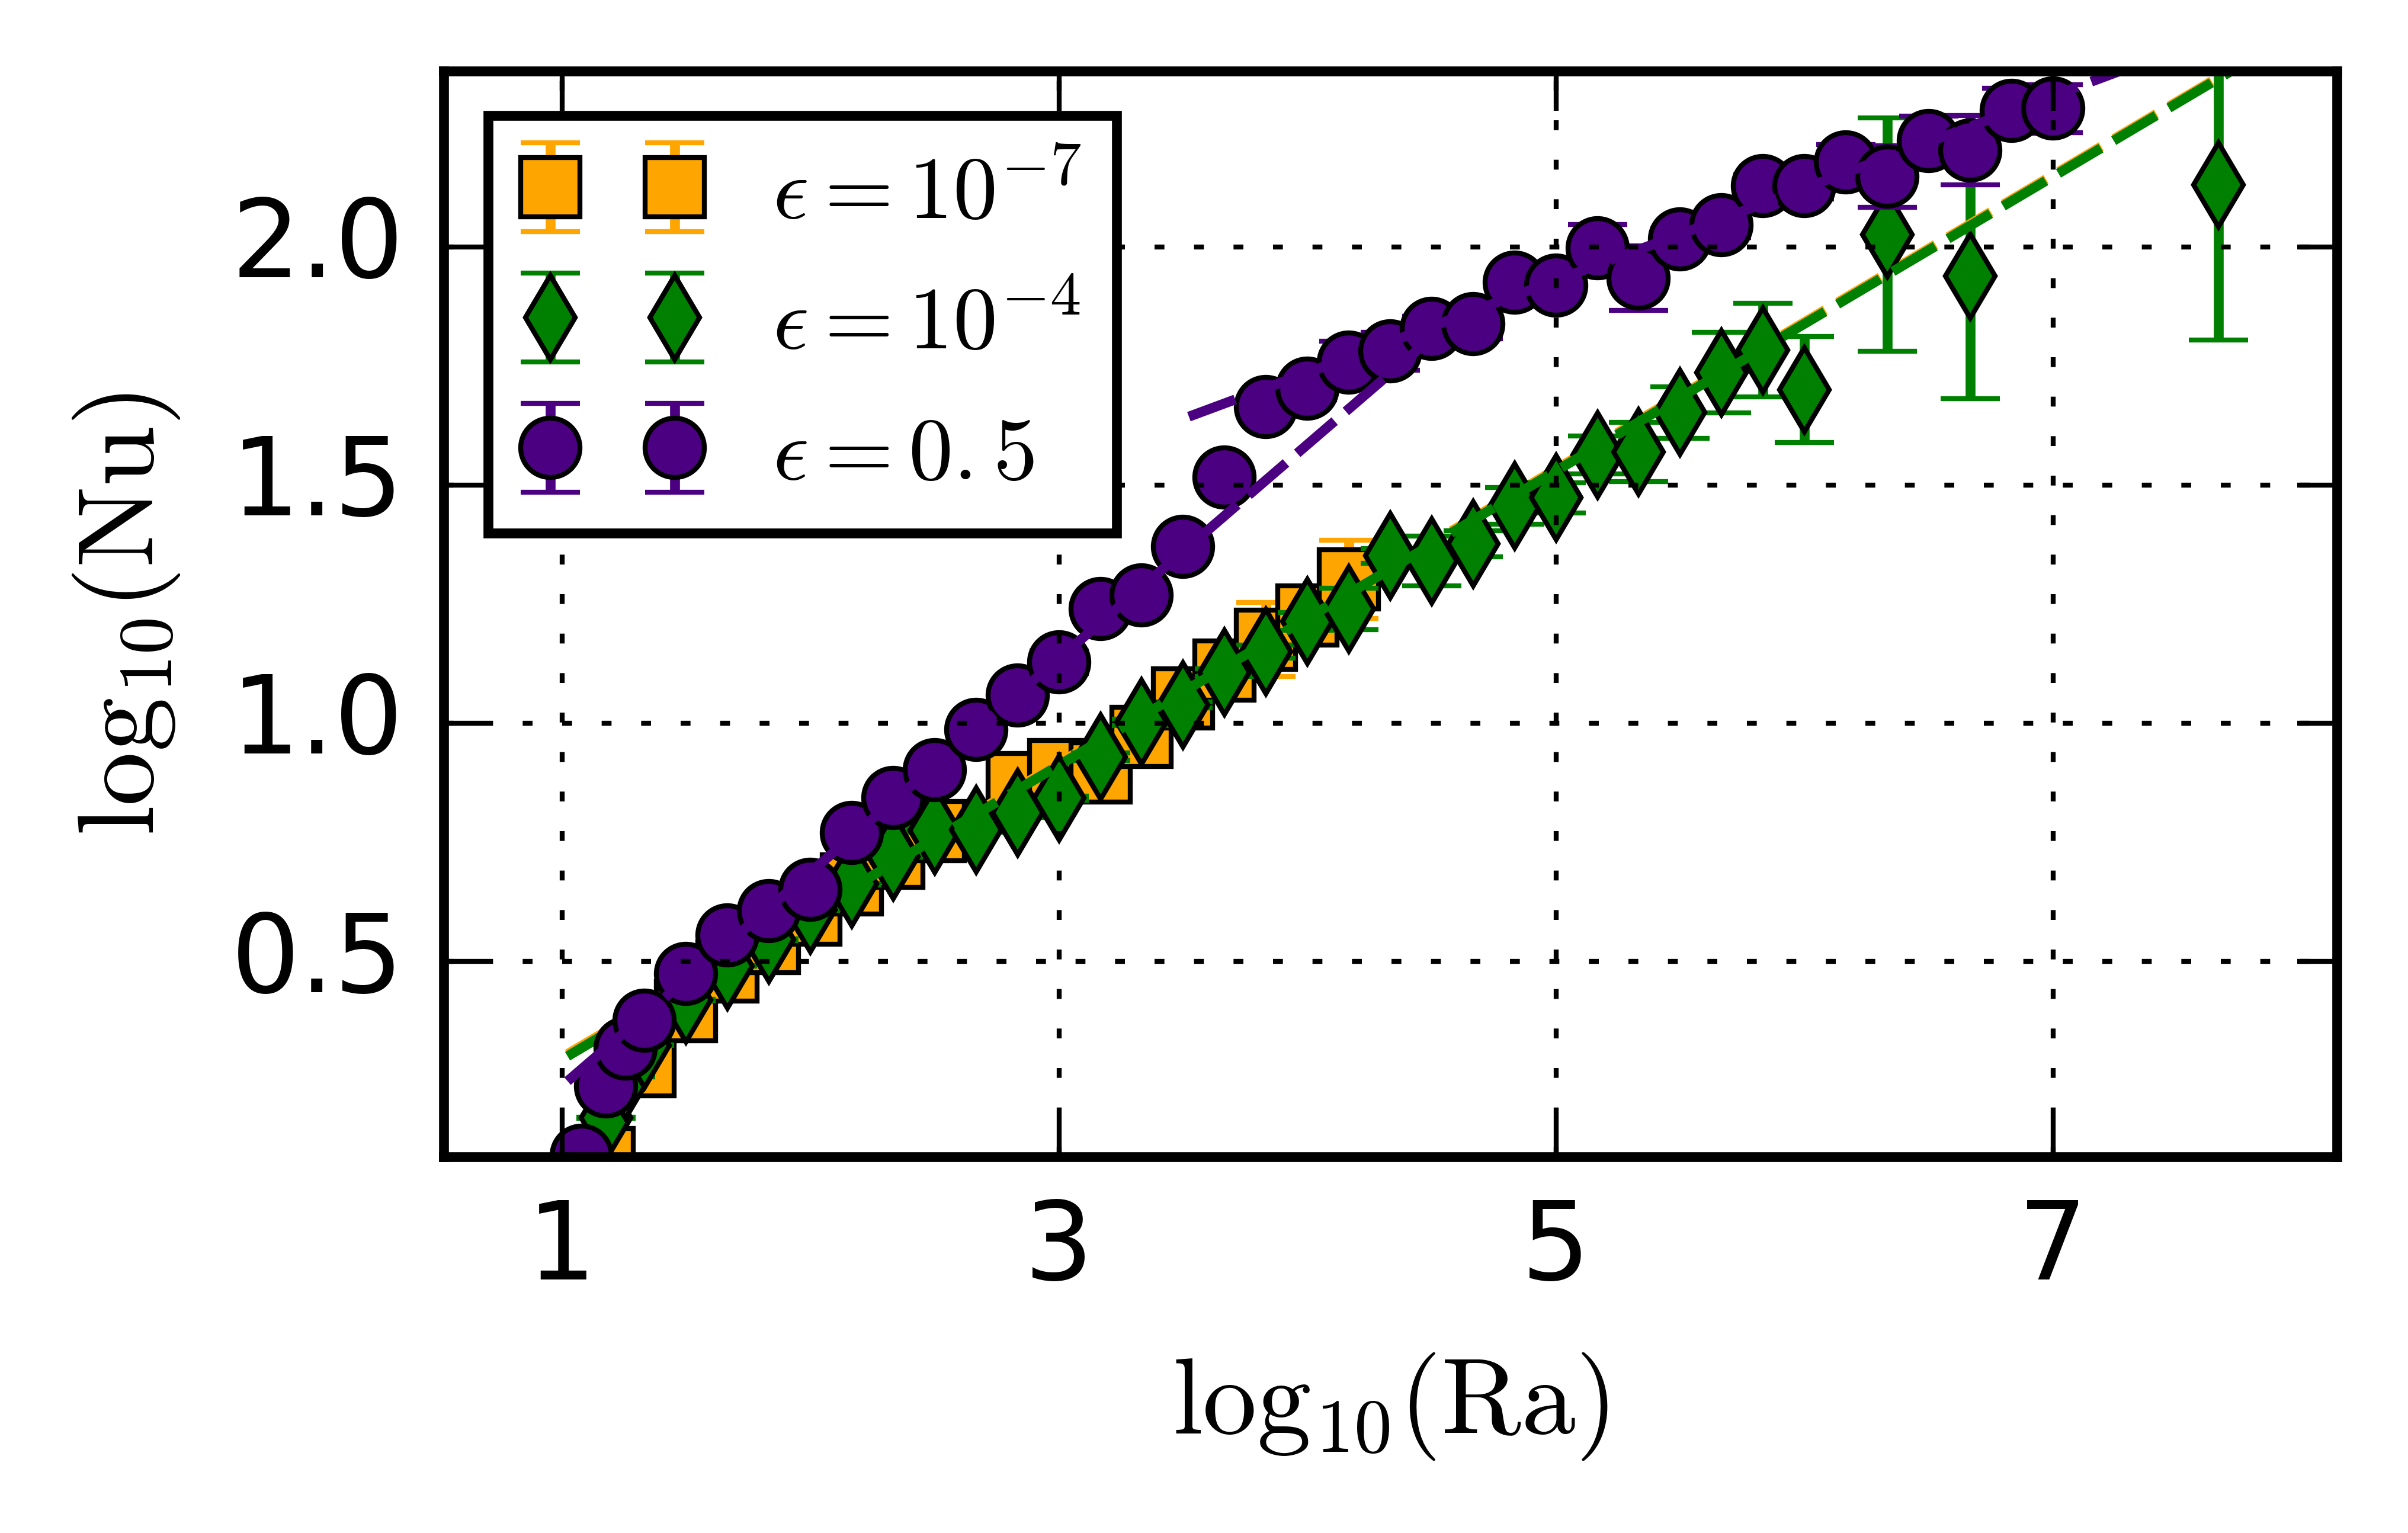
\includegraphics[width=3.5in]{./figs/nu_v_ra.eps}
\caption{Variation of the Nusselt number as a function of the Rayleigh number is shown.
\label{fig:nu_v_ra} }
\end{figure}




\begin{acknowledgements}
This work was supported by the CU/NSO Hale Graduate Fellowship and Juri's allocation and Ben's allocation.
\end{acknowledgements}

\bibliography{../biblio.bib}
\end{document}
